\documentclass[11pt,twocolumn]{article}

\usepackage{times}
\usepackage{fullpage}

\usepackage{booktabs}  % for \midrule
%\usepackage{subfigure}
\usepackage{balance}
\usepackage{graphicx}
\usepackage{xspace}
%\usepackage{pslatex}
%\usepackage{pifont}
%\usepackage{multirow}
%\usepackage{array}
%\usepackage{booktabs}
%\usepackage{cite}
\usepackage{url}
%\usepackage{cancel}
\usepackage{color,colortbl}
%\usepackage{microtype}
%\usepackage{textcomp}% http://ctan.org/pkg/textcomp
\usepackage{tabularx}
\usepackage{framed}
\usepackage[]{algorithm2e}
\SetAlFnt{\small}
\SetAlCapFnt{\small}
\usepackage{algorithmic}

\usepackage{listings}
%\usepackage{scrextend}
%\usepackage{mathtools}
\usepackage{pbox}

\let\labelindent\relax
\usepackage{enumitem}

\usepackage{tikz}
\usetikzlibrary{arrows,automata}
\usetikzlibrary{calc,positioning}
\usepackage{lipsum,adjustbox}

%\usepackage{tikz}
%\usepackage{decorations.pathmorphing}
%\usepackage{assymb}

\usepackage[labelfont=bf]{caption}

%\theoremstyle{plain}
\newtheorem{theorem}{\bf{Theorem}}%[section]
\newtheorem{lemma}[theorem]{\bf{Lemma}}
\newtheorem{corollary}[theorem]{\bf{Corollary}}
\newtheorem{proofl}[theorem]{\bf{Proof}}
\newtheorem{proposition}[theorem]{\bf{Proposition}}

%\theoremstyle{definition}
\newtheorem{definition}{\bf{Definition}}%[section]
\newtheorem{observation}{\bf{Observation}}%[section] 

%\theoremstyle{remark}
\newtheorem{example}{\bf{Example}}
\newtheorem{notation}{\bf{Notation}}
\newtheorem{fact}{\bf{Fact}}

\usepackage{listings}
%%\usepackage{listings-golang}
\usepackage{color}

%\usepackage{sectsty}
%\sectionfont{\fontsize{12}{15}\selectfont}

\usepackage{hyperref}


\newcommand\mypara[1]{\vspace{.3em}\noindent\textbf{#1}}
\newcommand{\urlwofont}[1]{\urlstyle{same}\url{#1}}


%%%%%%%%%%%%%%%%%%%%%%%%%%%%%%%%%%%%%%%%
% Useful reviewing/feedback annotations
\usepackage{ifthen}
\usepackage[normalem]{ulem} % for \sout
\usepackage{xcolor}
\usepackage{amssymb}

\newcommand{\ra}{$\rightarrow$}
\newboolean{showedits}
\setboolean{showedits}{true} % toggle to show or hide edits
\ifthenelse{\boolean{showedits}}
{
	\newcommand{\ugh}[1]{\textcolor{red}{\uwave{#1}}} % please rephrase
	\newcommand{\ins}[1]{\textcolor{blue}{\uline{#1}}} % please insert
	\newcommand{\del}[1]{\textcolor{red}{\sout{#1}}} % please delete
	\newcommand{\chg}[2]{\textcolor{red}{\sout{#1}}{\ra}\textcolor{blue}{\uline{#2}}} % please change
}{
	\newcommand{\ugh}[1]{#1} % please rephrase
	\newcommand{\ins}[1]{#1} % please insert
	\newcommand{\del}[1]{} % please delete
	\newcommand{\chg}[2]{#2}
}

\newboolean{showcomments}
\setboolean{showcomments}{true}
%\setboolean{showcomments}{false}
\newcommand{\id}[1]{$-$Id: scgPaper.tex 32478 2010-04-29 09:11:32Z oscar $-$}
\newcommand{\yellowbox}[1]{\fcolorbox{gray}{yellow}{\bfseries\sffamily\scriptsize#1}}
\newcommand{\triangles}[1]{{\sf\small$\blacktriangleright$\textit{#1}$\blacktriangleleft$}}
\ifthenelse{\boolean{showcomments}}
%{\newcommand{\nb}[2]{{\yellowbox{#1}\triangles{#2}}}
{\newcommand{\nbc}[3]{
 {\colorbox{#3}{\bfseries\sffamily\scriptsize\textcolor{white}{#1}}}
 {\textcolor{#3}{\sf\small$\blacktriangleright$\textit{#2}$\blacktriangleleft$}}}
 \newcommand{\version}{\emph{\scriptsize\id}}}
{\newcommand{\nbc}[3]{}
 \renewcommand{\ugh}[1]{#1} % please rephrase
 \renewcommand{\ins}[1]{#1} % please insert
 \renewcommand{\del}[1]{} % please delete
 \renewcommand{\chg}[2]{#2} % please change
 \newcommand{\version}{}}
\newcommand{\nb}[2]{\nbc{#1}{#2}{orange}}

\definecolor{ibcolor}{rgb}{0.4,0.6,0.2}
\newcommand\iv[1]{\nbc{IB}{#1}{ibcolor}}
\usepackage{wasysym}
\newcommand\yesml[1]{\nbc{ML {\textcolor{yellow}\sun}}{#1}{mircolor}}

\definecolor{sgcolor}{rgb}{0.2,0.0,0.5}
\newcommand\sg[1]{\nbc{SG}{#1}{sgcolor}}

\definecolor{samcolor}{rgb}{0.2,0.4,0.2}
\newcommand\sam[1]{\nbc{SC}{#1}{samcolor}}

\definecolor{hccolor}{rgb}{0.21,0.54,0.84}
\newcommand\hc[1]{\nbc{HC}{#1}{hccolor}}

\definecolor{ideacolor}{rgb}{1.0,0,0.5}
\newcommand\idea[1]{\nbc{IDEA}{#1}{ideacolor}}


\definecolor{abstractcolor}{rgb}{0.0,0.5,1.0}
\newcommand\rabstract[1]{\nbc{ABSTRACT}{#1}{abstractcolor}}

\definecolor{introcolor}{rgb}{0.0,1.0,0.5}
\newcommand\rintro[1]{\nbc{INTRO}{#1}{introcolor}}

\definecolor{papercolor}{rgb}{1.0,1.0,0.0}
\newcommand\rpaper[1]{\nbc{PAPER}{#1}{papercolor}}

\definecolor{multicolor}{rgb}{1.0,0,0}
\newcommand\rmulti[1]{\nbc{MULTI}{#1}{multicolor}}

% Todo Command
\definecolor{todocolor}{rgb}{0.9,0.1,0.1}
\newcommand{\todo}[1]{\nbc{TODO}{#1}{todocolor}}


%%%%%%%%%%%%%%%%%%%%%%%%%%%%%%%%%%%%%%%%


\begin{document}

%\title{Inferring likely data invariants of distributed systems}
\title{Balanced Distributed Graph Processing}
\author{Anil Yelam, Audrey Randall}
\date{}

\maketitle

\begin{abstract}
\label{sec:abstract}
\small
\textit{In big data analytics, balanced execution of a computation is important for maximizing 
utilization of available resources in the cluster like CPU, Memory and Network. Various
works in the past have looked at optimized execution of big data platforms like Apache 
Hadoop MapReduce, Apache Spark and other sort and shuffle based workloads. In this paper,
we go on a similar quest for graph processing frameworks, which are equally commonly used
in big data processing and has not been hitherto well studied. We discuss various 
factors that affect the balanced execution of a graph processing algorithms on a given 
cluster. Specifically, we focus on the effect of different graph partitioning methods 
on performance of Pagerank algorithm on a wide range of natural graphs. By both studying 
the properties of these graphs and results from the pagerank runs on Apache Giraph, we show 
that even the simplest of the partitioning schemes can have a significant effect on the 
performance.}
\end{abstract}

\section{Introduction}
\label{sec:intro}
The importance of balanced execution of big data frameworks (Papers to link: 
Osterhout\cite{Ousterhout:2015:MSP:2789770.2789791}, Themis\cite{Rasmussen:2012:TIM:2391229.2391242}, 
TritonSort\cite{Rasmussen:2013:TBE:2427631.2427634}).

Why we picked graph processing.

What we did or found out, in a nutshell.


\section{Background}
\label{sec:background}

All about the graph processing frameworks and their computational models, basically 
a brief summary of \cite{Heidari:2018:SGP:3212709.3199523}. And a bunch of related 
papers we have read, like comparison papers \cite{Guo:2014:WGP:2650283.2650530,
Ammar:2018:EAD:3231751.3242935} and some earlier graph processing systems these papers 
point to - such as Pregel\cite{Malewicz:2010:PSL:1807167.1807184}, PowerGraph
\cite{Gonzalez:2012:PDG:2387880.2387883} and others.





\section{Discussion}
\label{sec:discussion}

Of the features of graph processing frameworks discussed in the last section,
input partitioning seems like the one that effects the performance significanlty 
- so we decided to focus on that in this paper. As we limit ourselves to vertex-centric models, 
we only focus on vertex partitioning methods. There are two potential ways in which the 
partitioning affects performance:
\begin{itemize}
    \item \textbf{The distribution of edges across partitions} Given that the computational complexity 
    of most graph algorithms is on the order of number of edges, the share of each worker in the 
    computation depends on number of edges its partition has. In order to avoid stragglers 
    (especially for synchronous coordination frameworks like Giraph), the partitioning scheme
    should distribute the edges evenly and try to minimize the variation in the number of edges 
    across partitions.
    \item \textbf{The fraction of inter-partition edges} As vertex partitioning puts vertices
    in different partitions, a lot of edges may end up with their vertices in different 
    partitions - we call these inter-partition edges. As graph algorithms work by sending 
    messages over edges, messages sent over these inter-partition edges need to be sent across network
    and add to a lot of performance overhead. A good partitioning scheme tries to minimize the 
    number of inter-partition edges. Finding such an optimal partitioning is an NP-complete problem, 
    so we can only go with heuristics.
\end{itemize}

The partitioning heuristics can be as simple as hash-based ones that hash vertices into buckers 
without regard to their connectivity or complex ones that try to reduce the edge cuts across partitions 
\cite{Salihoglu1} that comes at added computational overhead of partitioning itself. Our intial goal 
was to implement a mix of simple and complex partitioning heuristics and evaluate the tradeoff between
performance benefits of good partitioning versus the overhead of partitioning itself. However, due to 
limited time and the complexity of implementing these heuristics on Apache Giraph, we restricted 
ourselves to evaluating two simple yet very different partitioning schemes that does not incur any 
computational overhead:
\begin{itemize}
    \item \textbf{Round-robin Partitioning} In this method of partitioning, we assign each vertex to 
    partition on a round-robin basis (we use modulo operator on vertex id to acheive this). The idea 
    is that for a graph with vertices indexed according to certain traversal algorithm, each partition 
    would get vertices from all over the graph in a uniform way.
    \item \textbf{Range Partitioning} In this one, we divide the vertex index space into equal ranges
    (number of ranges being number of partitions required) and vertices from each range is assigned to 
    each partition. This partitioning roughly divides the graph spatially and so partitions will exhibit 
    better locality.
\end{itemize}

Since these partitioning methods are straight-forward, we first perform a theoretical analysis of our 
input graphs to see the distribution of edges in and across partitions, which is presented in the 
next section. Later, we run PageRank 
algorithm on these graphs using Giraph and analyze the running times to see if our observations 
hold in practice.





\subsection{Apache Giraph}
\label{sec:giraph}

Apache Giraph\cite{ApacheGiraph} is a popular open-source implementation of
Pregel\cite{Malewicz:2010:PSL:1807167.1807184}. Giraph runs on Hadoop MapReduce and uses 
Map-only jobs to schedule and coordinate the 
vertex-centric workers and uses HDFS for storing and accessing graph datasets. 
It is developed in Java and has a large community of developers and users such as 
Facebook\cite{GiraphAtFacebook}. Giraph has a faster input loading time compared to Pregel 
because of using byte array for graph storage. On the other hand, this method 
is not efficient for graph mutations, which lead to decentralized edges when removing an edge. 
Giraph inherits the benefits and deficiencies of the Pregel vertex-centric
programming model. We picked Giraph for the supposed ease of use of this framework and the 
community support. 

We ran Giraph on a 4-node hadoop cluster. Each of these nodes are t2.xlarge AWS machines
each with 4 vCPUs, 16 GB Memory, 32 GB SSD and upto 1 Gbps Network. Giraph workers run 
as Map jobs, each in their YARN containers. YARN allows setting limits on the number of cores 
and memory to each container, so we limit each giraph worker to 1 vcore and 2 GB memory - so 
we could run a maximum of around 20 giraph workers given our cluster capacity. 
We chose PageRank as our graph algorithm since it is global and involves computation at all the vertices 
and  edges in every iteration. We ran five iterations of PageRank (called SuperSteps) on each 
graph, with the two partitioners that we implemented in Giraph  using \textit{HashPartitionerFactory} 
and \textit{SimpleLongRangePartitionerFactory} classes. The CPU usage on all the machines 
from a sample run of Giraph using round-robin partitioning on Facebook's Darwini graphs 
is shown in Figure \ref{fig:sample_giraph_run}.

\begin{figure}
	\centering
	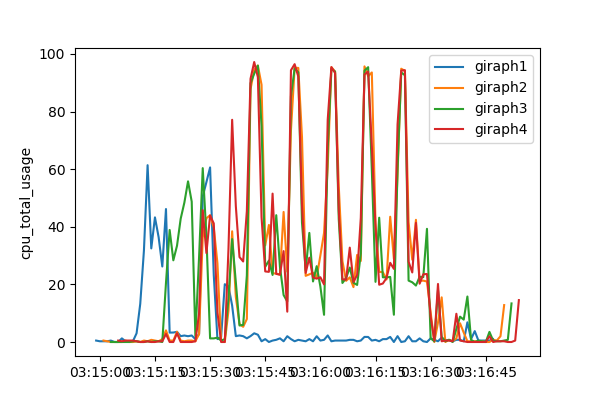
\includegraphics[width=\columnwidth]{./samplerun.png}
    \caption{CPU usage on all the nodes from a sample PageRank run over time. The five spikes 
        indicate five iterations of the algorithm.}
	\label{fig:sample_giraph_run}
\end{figure}

A significant amount of the time spent on this project was spent setting up our cluster and installing 
Giraph and all of its dependencies. Even for a well-supported and widely used piece of software like 
Giraph, this was a time consuming challenge. To begin with, version mismatches of Java, HDFS, Ubuntu, 
and Giraph itself caused a number of difficult-to-debug errors. For example, installing the most recent 
version of Java caused a mysterious build error that took hours to track down a workaround for (the workaround 
being to downgrade Java). Additionally, once Giraph had been successfully built, we spent eight 
hours tuning various settings before the example job provided in the documentation would run without error. 
This was due to a number of factors. First, configuration settings are scattered across many different files, 
making it challenging to identify the source of a problem and difficult to predict how the settings would interact 
with each other. Second, few facilities existed for fine-tuning resource allocation. Many jobs failed with 
``out of memory'' exceptions because it was difficult to tune the amount of memory they would be 
allocated. Third, error messages are not gathered in a central location - the existence of numerous log files made 
tracking down errors time consuming. Finally, Giraph seems to be a highly sensitive and delicate system. 
Unfortunately, as a result it is fragile: the slightest misallocation or imbalance of a resource causes jobs to 
fail with little explanation.

Given limited total memory capacity of our cluster (4*16 GB), we could only run medium sized graphs 
(with around 100 million edges) as Giraph does everything in memory. We ran PageRank on each of the graphs 
we discussed in previous section with both round-robin and range partitioners while varying the number of 
giraph workers (each with 2 GB memory) from 2 to 20. The execution times (excluding any preprocessing time) 
for these graphs using different partitioners are shown in Figures 
\ref{fig:giraph_roundrobin} and 
\ref{fig:giraph_range}. The missing data points for few input graphs at 2, 4 and 6 workers is due to the fact 
that these graphs are too big and cannot be run with fewer workers. 


\begin{figure}[!t]
	\centering
	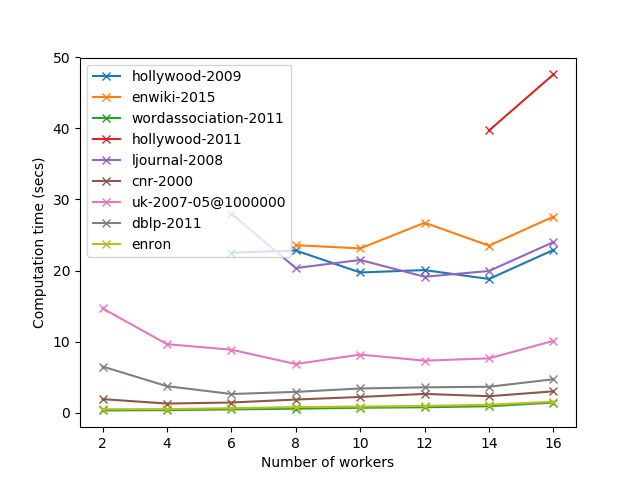
\includegraphics[width=\columnwidth]{./giraph_roundrobin.png}
    \caption{PageRank computation time for various graphs on Giraph with RoundRobin vertex partitioner
        as number of workers (partitions) are increased.}
	\label{fig:giraph_roundrobin}
\end{figure}

\begin{figure}[!t]
	\centering
	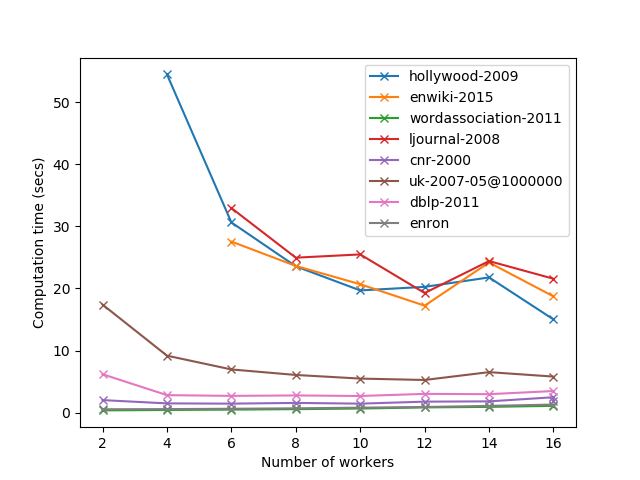
\includegraphics[width=\columnwidth]{./giraph_range.png}
    \caption{PageRank computation time for various graphs on Giraph with Range vertex partitioner
    as number of workers (partitions) are increased.}
	\label{fig:giraph_range}
\end{figure}

In both cases, we expected the computational time to go down as the number of workers increased, 
which only happened with the range partitioner. Computation times for range partitioner are less 
compared to round-robin partitioner for every graph, which seems to indicate that network overhead 
affects the performance more than straggler problems caused by the imbalance in partitioning.
In general, we didn't see the results we were expecting. Our conclusion was that Giraph has a 
lot of setup and preprocessing overheads that adds a lot of 
noise that significantly affects our runs since we use medium sized graphs that take only few seconds 
to run. We believe that 
using much larger graphs (like Twitter or Facebook) would give us the results that could let us 
clearly draw conclusions, but we could not run them due to resource limitations. We leave that to 
future work.

\section{Results}
\label{sec:eval}

\subsection{Input Graph Characteristics}

\begin{table*}[t]
	\centering
	\begin{tabular}{r|cccl}
		\textbf{Name} & \textbf{Vertices} & \textbf{Edges} & \textbf{Vertex 
			means...} & \textbf{Edge means...}\\
		\hline
		cnr-2000 & 325557 & 3216152 & Website & Hyperlink\\
		dblp-2011 & 986324 & 6707236 & Scientist & Paper collaboration \\
		enron & 69244 & 276143 & Person & Recipient of email\\
		wordassociation-2011 & 10617 & 72172 & Word & Interpreted association \\
		hollywood-2011 & 2180759 & 228985632 & Actor & Appearance in movie\\
		hollywood-2009 & 1139905 & 113891327 & Actor & Appearance in movie\\
		ljournal-2008 & 5363260 & 79023142 & User & Friend\\
		uk-2007-05@1000000 & 1000000 & 41247159 & Website & Hyperlink\\
		twitter & 41652230 & 1468365182 & User & Follower\\
		uk-2002 & 18520486 & 298113762 & Website & Hyperlink\\
	\end{tabular}
	\caption{Details of graph datasets}
	\label{tab:graph_types}
\end{table*}

\begin{figure}
	\centering
	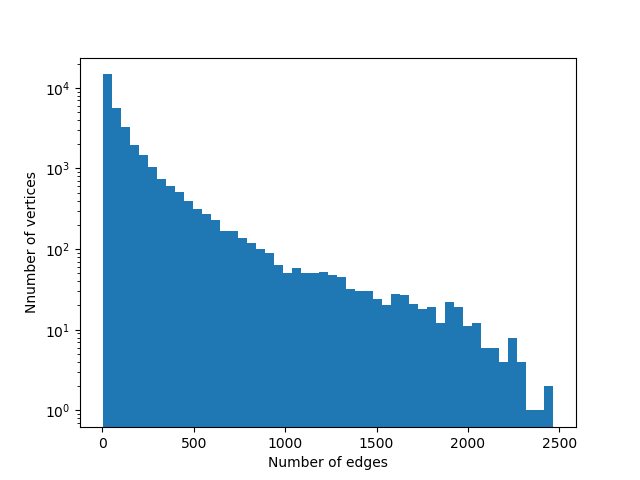
\includegraphics[width=\columnwidth]{../good_plots/degree_distribution_10_mil.png}
	\caption{Degree distribution for a representative graph in our dataset, 
		demonstrating that the graphs we chose are power-law graphs.}
	\label{fig:degree_distribution}
\end{figure}

We selected eleven graphs to analyze. Although we originally chose several 
others, we were limited by the hardware we had the funds to rent to analyzing 
relatively small graphs. A tradeoff exists between the size of a graph, the 
number of workers assigned to handle its vertices, and the amount of memory on 
a server. First, there is a minimum amount of memory that a Giraph worker 
requires in 
order to run. This puts an upper bound on the number of workers that can be run 
on any machine. Second, there appears to be a minimum number of workers that 
can be assigned to a graph of a given size in Giraph: when too few are 
assigned, the job fails. Presumably, this is because each worker can only 
feasibly handle a certain number of vertices, although it is unclear why Giraph 
chooses to terminate jobs rather than allowing them to eventually complete. 
This factor puts a lower bound on the number of workers that can be assigned to 
a graph, which is dependent on the size of the graph. Given these constraints, 
we restricted ourselves to graphs with approximately 200 million edges or fewer.

Our graphs came from the Laboratory for Web Algorithmics (LAW)
\cite{BoVWFI, BRSLLP}. We considered using artificial graphs generated by 
Facebook's Darwini project \cite{edunov_darwini:_2016}, but eventually 
concluded that they were too large. The LAW graphs come 
from a variety of places. We selected a diverse subset of them, as shown in 
Table \ref{tab:graph_types}.

We also paid attention to the distribution of the degrees of the vertices in 
the graphs that we chose. Since most natural graphs are power-law distributed, 
our graphs primarily follow that pattern. Figure \ref{fig:degree_distribution} 
shows a representative example of the degree distribution of a graph in our 
dataset. 

\begin{figure}[!t]
	\centering
	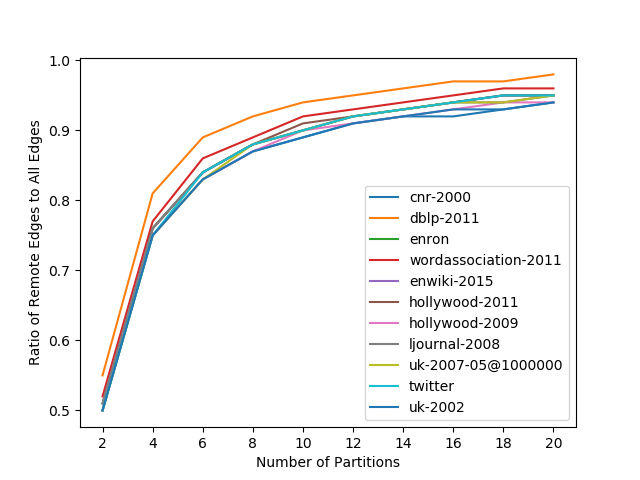
\includegraphics[width=\columnwidth]{../good_plots/remote_to_all_modulo.png}
	\caption{Ratio of remote edges (requiring messages to be sent across the 
	network) to all edges for various numbers of partitions, where partitioning 
	is done by taking the modulus of the vertex ID and number of workers.}
	\label{fig:remote_to_all_mod}
\end{figure}

\begin{figure}[!t]
	\centering
	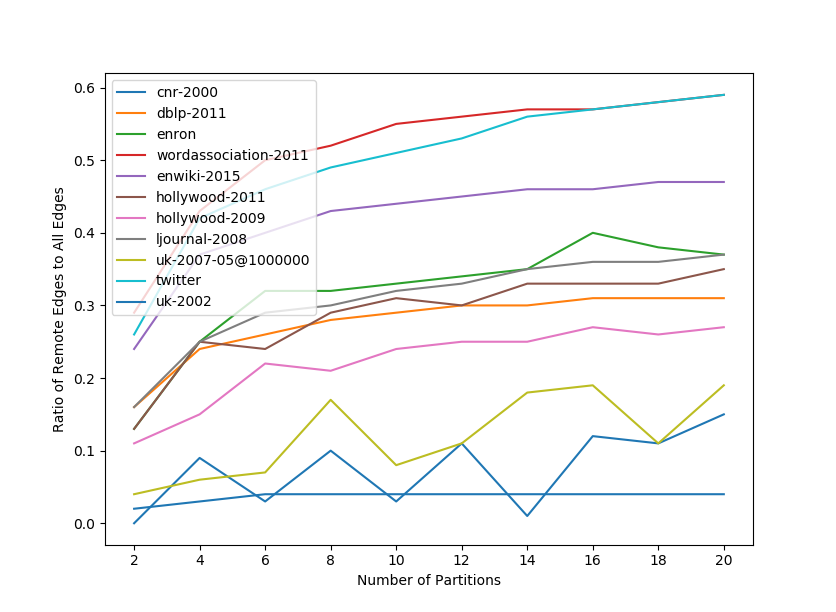
\includegraphics[width=\columnwidth]{../good_plots/remote_to_all_chunked.png}
	\caption{Ratio of remote edges to all edges for various numbers of 
		partitions, where range partitioning is used.}
	\label{fig:remote_to_all_range}
\end{figure}

We ran experiments to look at two metrics that we believe are predictors of 
performance: the number of edges given to each worker that require network 
requests, and the range of the number of edges given to each worker. We chose 
the first metric because we predict that if a worker is assigned a high 
proportion of edges that require it to make network requests, the time taken to 
run each step of computation will be much higher. Recall that in PageRank, 
every computational step requires a message to be sent along every edge. If 
that message begins and ends at vertices that are stored on the same machine, 
the overhead is much lower than it would be if the source and destination 
vertices are stored on two separate machines, thus necessitating a network 
request. Therefore, we measure the ratio between the number of local edges and 
the total edges assigned to a worker for various numbers of partitions and two 
partitioning schemes. Figures \ref{fig:remote_to_all_mod} and 
\ref{fig:remote_to_all_range} show the results.

Figure \ref{fig:remote_to_all_mod} shows the partitioning scheme where vertices 
are assigned to workers by taking the modulo of their vertex ID with the number 
of workers in the cluster. Figure \ref{fig:remote_to_all_range} shows the 
results of ranged partitioning. We hypothesized that both partitioning schemes 
would yield a graph similar to Figure \ref{fig:remote_to_all_mod}, because if 
vertices are truly randomly assigned, then there is a greater chance of a 
vertex being assigned to a remote worker than a local one as the number of 
workers increases. However, range partitioning is not random - it takes 
locality into account. The graphs we analyze are taken from real-world 
data. Since they have to 
be created by some sort of crawler or traversal algorithm, they exhibit a 
certain amount of locality. Range partitioning therefore
does a significantly better job than modulo partitioning at reducing the 
fraction of remote edges to local edges, as shown in Figure 
\ref{fig:remote_to_all_range}.

The second predictor of performance that we measured was the variation of the 
number of edges assigned to each worker. We assigned an equal number of 
vertices to each worker with all of our partitioning schemes, but this did not 
guarantee that the number of edges was the same. To our surprise, large graphs 
tend to approach edge equanimity even with the simple partitioning algorithms 
we use, which make no attempt to assign edges equally. We quantified this 
relationship in terms of the coefficient of variation of the number of edges 
assigned to each worker, for a varied number of workers, as shown in Figures 
\ref{fig:cv_mod} and \ref{fig:cv_range}.

\begin{figure}[!t]
	\centering
	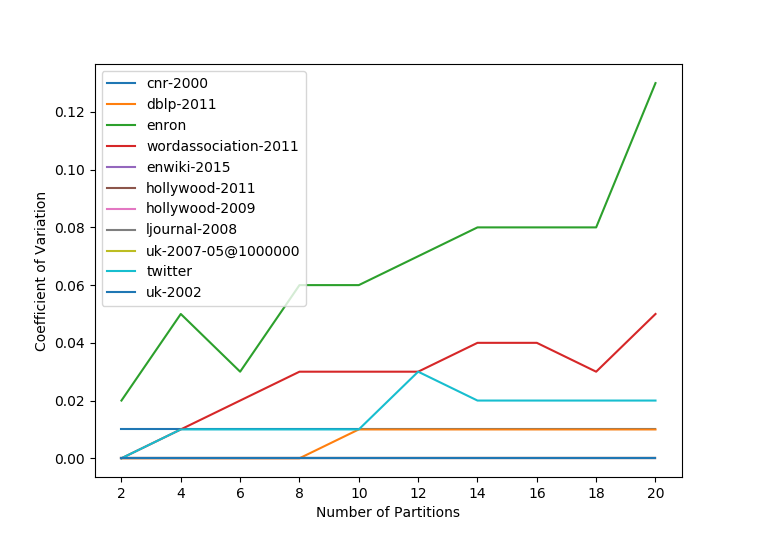
\includegraphics[width=\columnwidth]{../good_plots/range_as_cv_modulo.png}
	\caption{Range of the maximum number of edges handled by each worker to the 
		minimum handled by any worker, expressed by the coefficient of 
		variation, 
		for various numbers of partitions, with modulo partitioning.}
	\label{fig:cv_mod}
\end{figure}

\begin{figure}[!t]
	\centering
	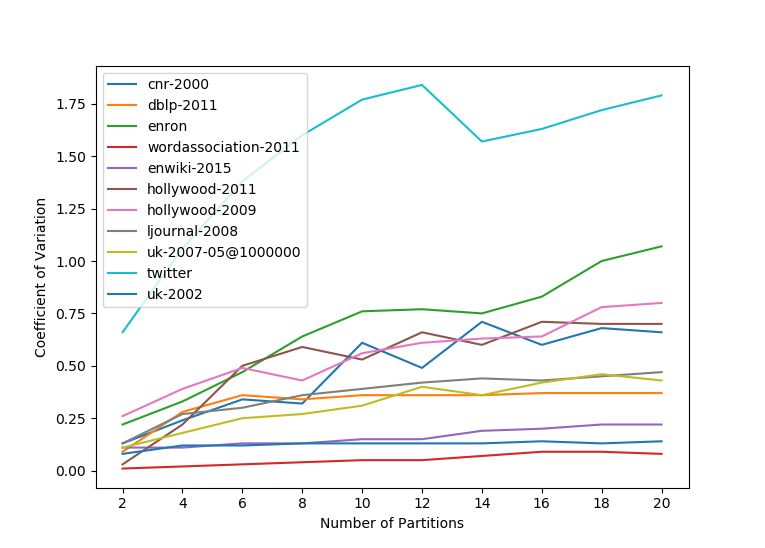
\includegraphics[width=\columnwidth]{../good_plots/range_as_cv_chunked.png}
	\caption{Range of the maximum number of edges handled by each worker to the 
		minimum handled by any worker, expressed by the coefficient of 
		variation, for various numbers of partitions, with range 
		partitioning.}
	\label{fig:cv_range}
\end{figure}

Figure \ref{fig:cv_range} shows that range partitioning led to a significantly 
higher 
difference between the number of edges assigned to each worker. This is likely 
due to locality again - range partitioning tends to capture any clustering 
present in the graph, whereas modulo partitioning evenly distributes clusters 
and breaks them up. One graph in particular stood out from the others: twitter, 
which draws edges between followers on the Twitter social network. Twitter is 
the largest graph we analyze, but large graphs do not necessarily appear to 
correspond to high coefficients of variation when it comes to edge 
distribution. It is possible that the twitter graph has more severe clustering 
than the other graphs, but why it should be so much higher than (for example) 
another social network graph like ljournal-2008, we do not know. Figure 
\ref{fig:cv_mod} shows a lower range of number of edges assigned to each 
worker, perhaps because modulo partitioning is closer to completely random than 
range partitioning. Here, many graphs have such even edge partitioning that 
their coefficient of variation is zero for all numbers of partitions. 

Our takeaway from these experiments is that there is a tradeoff to be made when 
choosing a partitioning algorithm. If a particular job is concerned with having 
workers that lag behind the fastest workers in the cluster, it is probably 
important to choose to distribute edges as well as vertices evenly among the 
workers, and modulo partitioning should be used. If a job is likely to be 
network bound, range partitioning may be more effective, since it leverages 
locality to reduce the number of remote edges each worker must handle.
\section{Conclusion}

We present a small study on the effects of partitioning algorithms on 
performance predictors (such as the distribution of edges on workers) and 
performance itself on Apache Giraph. We conclude that a tradeoff exists between 
reducing the number of messages that must be sent over the network and 
equalizing the number of edges that are distributed to each node: to optimize 
the former, range partitioning should be used, and to optimize the latter, 
modulo partitioning is best. 
%% Add other sections here


\balance
\vspace{-0.3cm}
{\footnotesize \bibliographystyle{acm}
\bibliography{paper}}
\vspace{-0.5cm}

\end{document}
